\documentclass{article}
\usepackage[utf8]{inputenc}
\usepackage[spanish, es-tabla]{babel}
\usepackage{hyperref}
\usepackage{cite} 
\usepackage{graphicx} 


\title{Plataforma microfluídicas capilares.\\Una buena combianción.}
\author {Miguel M Erenas, Fermin Capitán Vallvey e Ignacio de Orbe-Payá\\
Dpto. Química Analítica. Universidad de Granada}




\begin{document}
	\maketitle
\begin{abstract}
URL repositorio: \url{https://github.com/Obiblion/proyecto_final}\\
Dentro de los dispositivos Point-of-Care (POC), los sensores microfluídicos se caracterizan por utilizar pequeños volúmenes tanto de muestra como de reactivos necesarios para acometer su función. Existen dispositivos microfluídicos que utilizan diferentes materiales como soporte, que los dotan de una serie de características específicas. El material más utilizado en la actualidad es el papel, aunque recientemente se están comenzando a usar nuevos soportes como hilo o tela de algodón.  
\end{abstract}
\textbf{Keywords}: Smaprtphone, $\mu$PAD, $\mu$CAD y $\mu$TAD



	
\section{Introducción}
Desde los primeros artículos que aparecieron en 2008\cite{Abe2008,Martinez2010} ha ido aumentando el interés por las plataformas capilares basadas en papel, hilo o tela. Estos dispositivos que no requieren soporte instrumental, son básicamente desechables y de un solo uso, presentan un enorme potencial de aplicación para la realización de medidas químicas a muy bajo coste compatibles con procesamiento TIC de las señales utilizando herramientas como smartphones.\\
 
El uso de papel tiene gran número de ventajas siendo una de las principales el que permite el movimiento de líquidos por capilaridad\cite{Cate2015}, aunque para ello es necesario definir el camino por el que debe de avanzar la muestra en disolución desde la zona de muestreo hasta la de detección atravesando zonas donde tienen lugar diferentes operaciones analíticas. Esto se resuelve mediante la fabricación de canales en el papel, donde se puede confinar el fluido en canales abiertos o cerrados y guiarlo de forma controlada a través del circuito\cite{Fenton2009}.\\
 
A pesar de ser el papel, al igual que la tela, un soporte que puede funcionalizarse con facilidad, presenta el inconveniente de la definición de canales y la dificultad de combinar diferentes tipos de papeles para llevar a cabo las operaciones analíticas necesarias. La búsqueda de nuevos materiales ha conducido al empleo de hilos. Debido a su estructura, formada por un conjunto de hebras helicoidalmente enrolladas, es posible el avance de las disoluciones de muestras y reactivos hasta la zona de detección debido a procesos de capilaridad en los espacios inter e intrafibras así como por el lumen\cite{Banerjee2013}. Por otra parte, el hilo permite la inmovilización de reactivos de diverso tipo\cite{Lu2015}. Aunque en principio el hilo es un soporte similar al papel, presenta una serie de ventajas diferenciales\cite{Nilghaz2013} pues no es necesario definir un camino a seguir como ocurre en papel y su flexibilidad y resistencia permite una mayor versatilidad y la posibilidad de diseñar sistemas 3D. Por otra parte, permite diseñar sistemas con hilos de diferente tipo, desde hidrofílicos como algodón hasta hidrofóbicos como seda. Por último, el menor volumen de muestra y reactivos necesarios junto el menor precio de los hilos respecto a papel, lo convierte en una alternativa de interés.\\

El uso de hilo como soporte para sistemas microfluídicos se propuso a finales de 2010\cite{Li2010} y desde entonces han aparecido no más de 40 artículos (Tabla\ref{tabla:biblio}) que han comenzado a desarrollar el concepto y establecer las características microfluídicas del soporte\cite{Ballerini2011}.
\begin{table}
	\centering
	\caption{Artículos publicados en los últimos años de dispositivos microfluídicos basados en papel, hilo y tela.}
	\label{tabla:biblio}
	
\begin{tabular}{|c|c|c|c|}
	\hline 
	Año & $\mu$PAD & $\mu$CAD & $\mu$TAD \\ 
	\hline 
	2019 & 177 & 6 & 3 \\ 
	\hline 
	2018 & 255 & 16 & 4 \\ 
	\hline 
	2017 & 213 & 7 & 6 \\ 
	\hline 
	2016 & 179 & 6 & 4 \\ 
	\hline 
	2015 & 155 & 5 & 6 \\ 
	\hline 
	2014 & 130 & 6 & 1 \\ 
	\hline 
	2013 & 98 & 5 & 0 \\ 
	\hline 
	2012 & 65 & 5 & 2 \\ 
	\hline 
	2011 & 27 & 3 & 1 \\ 
	\hline 
	2010 & 34 & 2 & 0 \\ 
	\hline 
	2009 & 10 & 0 & 0 \\ 
	\hline 
	2008 & 5 & 0 & 0 \\ 
	\hline 
\end{tabular} 
\end{table}

\section{Fabricación del dispositivo}

Para la preparación de los dispositivos microfluídicos en papel ($\mu$PAD) o en hilo ($\mu$TAD) hay que diseñar, en primer lugar, tanto el dispositivo como el accesorio en el que se va a situar, de forma que permita utilizarlo de forma sencilla y reproducible. El diseño debe considerar el área de recepción, los canales de transporte o separación y las áreas de detección, lo que dependerá del objetivo buscado con el dispositivo, el número de analitos a determinar, el número de réplicas, el volumen de muestra disponible, las operaciones analíticas a incluir y la química de reconocimiento a emplear.\\

Se han descrito diversas estrategias para la fabricación de dispositivos $\mu$PAD que se pueden resumir en dos: 1) por formación de barreras hidrofóbicas que delimiten los canales por deposición de materiales hidrofóbicos, así por bloqueo físico de poros (fotolitografia), por deposición de agentes hidrofobizantes (cera) o por modificación química de la celulosa (alquil cetena dímero) (Figura \ref{fig:papel}); 2) por recorte físico del papel con un plotter de corte o con un láser, obviando así la necesidad de construir canales\cite{Cate2015} (Figura \ref{fig:papel}).\\


%figura 1
\begin{figure}[h]
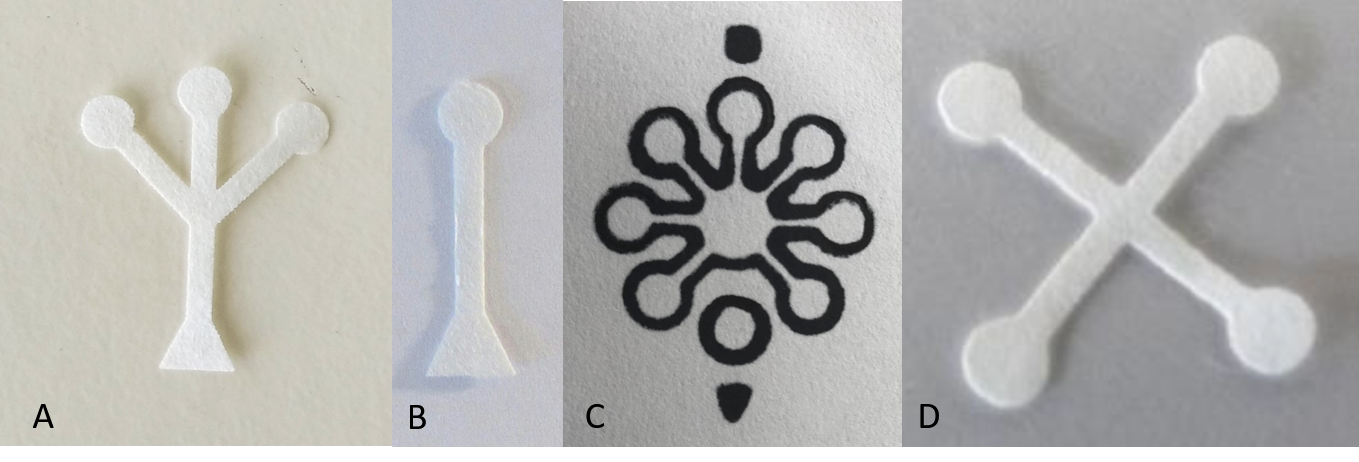
\includegraphics[width=\textwidth]{papel}
\caption{ $\mu$PAD fabricado con un plotter de corte, B y C) $\mu$PAD preparado con un láser de corte y D) $\mu$PAD impreso por tampografía}
\label{fig:papel}
\end{figure}

Del primer grupo de técnicas, se han descrito en bibliografía gran número de alternativas10, casi una por grupo. Un problema de este procedimiento de fabricación es la creación de una barrera hidrofóbica homogénea en todo el espesor del papel, pues cualquier pequeña fisura en la barrera provoca fugas que afectan a la eficiencia del $\mu$PAD. Nuestra experiencia se ha centrado en el estampado de patrones con tampones de PDMS impregnados en tinta hidrofóbica, serigrafía de los patrones en el papel mediante tintas vinílicas, serigrafía con cera e impresión del patrón mediante impresoras de tinta sólida basada en cera\cite{Lopez-Ruiz2014}. La impresión con ceras exige un posterior tratamiento térmico para fundirla. Todos estos procedimientos tienes una tasa de éxito que oscila entre el 60\% los primeros y el 80\% el último.\\ 

Otra estrategia seguida para el patronaje de los dispositivos es cortar la pieza de papel a usar mediante un plotter de corte o una impresora de corte láser. El plotter de corte funciona de manera similar a una impresora, pero en el cabezal lleva una cuchilla que corta el papel con la forma que definamos. El principal problema es que hay que adherir el papel sobre un soporte rígido y plano para realizar el corte del papel ya que se puede rasgar si no es así o si no está bien afilada la cuchilla. Como consecuencia, la tasa de éxito del proceso es del 75\% y el uso de cuchillas no permite fabricar dispositivos tan pequeños como otras metodologías, ya que cuanto más pequeño más se reduce la tasa de éxito.\\ 

Finalmente, otra aproximación al corte del papel es el uso de una impresora de corte láser, la cual nos permite realizar diseños similares a las de un plotter de corte, pero con ventajas como no tener que adherir el papel a un soporte rígido para poder cortarlo, presentando una tasa de éxito del 99\%. Además, permite hacer diseños mucho más pequeños gracias a la alta resolución que permite por lo que se puede considerar una buena opción para la fabricación de dispositivos $\mu$PAD. \\

En el caso de los dispositivos $\mu$TAD, no es necesario delimitar el canal a seguir por la muestra ya que viene definido por las propias fibras que componen el hilo. El proceso capilar en este caso se debe a que la disolución se va moviendo por los espacios interfibra del hilo avanzando a lo largo del mismo. Sin embargo, en el caso del algodón, las fibras que componen el hilo están recubiertas por ceras naturales lo que afecta al mojado del hilo y, por tanto, ralentizan e incluso impiden el proceso capilar. Por ello, es necesario llevar a cabo un tratamiento con plasma a vacío o alternativamente un proceso de limpieza con carbonato sódico para eliminar dichas ceras\cite{Nilghaz2013}.\\

%figura 2
\begin{figure}[h]
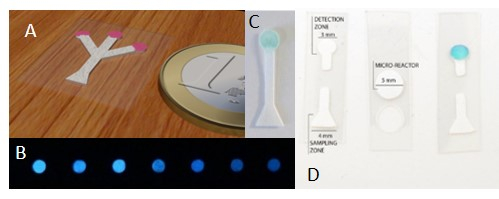
\includegraphics[width=\textwidth]{moneda}
\caption{Diferentes estrategias utilizadas para la fabricación de $\mu$PAD. A y B) Adheridos sobre cinta de doble cara; C) laminados; D) $\mu$PAD 3D compuesto de varios elementos, siendo uno de ellos reutilizable. }
\label{fig:moneda}
\end{figure}

Ya sea hilo o papel el soporte usado para el desarrollo del dispositivo microfluídico capilar, es necesario situarlos en algún tipo de soporte para facilitar su uso. Algunos de los procedimientos seguidos se muestran en las Figuras \ref{fig:moneda} y \ref{fig:hilo}. En el caso de dispositivos en papel, pueden laminarse, realmente es una encapsulación, habitualmente entre láminas de vinilo con un orificio correspondiente a la zona de muestreo (Figura \ref{fig:moneda}C); alternativamente, se puede adherir el dispositivo para su uso a cinta adhesiva de doble cara (Figura \ref{fig:papel}A). \\

En el caso de dispositivos basados en hilo se ha seguido en ocasiones una estrategia similar al papel, laminando entre sustratos flexibles. En la Figura \ref{fig:hilo}D se muestra un ejemplo de laminación de hilo con reactivos inmovilizados sobre una celda electroquímica serigrafiada. Otra posibilidad es el diseño de accesorios en metacrilato (Figura \ref{fig:hilo} A y C) que permiten mantener el hilo conteniendo las químicas de reconocimiento en una posición fija o bien coser el hilo en pequeños soportes de goma EVA que permita un fácil uso (Figura \ref{fig:hilo}B). De esta manera se evita que el hilo se retuerza al añadir la muestra por efecto del mojado dificultando la adquisición de imágenes y la medida de color.\\

Se ha iniciado el estudio de nuevos soportes para dispositivos microfluídicos como es el caso de tela de algodón ($\mu$CAD) preparando los patrones mediante serigrafía con tintas vinílicas o plastisol y posterior laminado tras inmovilizar la química necesaria. Por otra parte, el empleo de nanocelulosa depositada en el dispositivo grabado con impresora láser sobre láminas de metacrilato permite un rápido desplazamiento de la muestra, siendo una opción interesante (Figura \ref{fig:tela}).\\

%figura 3
\begin{figure}[h]
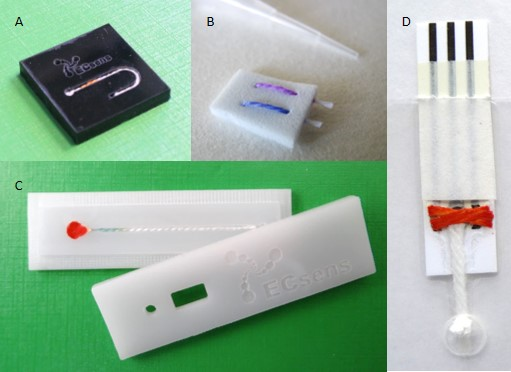
\includegraphics[width=\textwidth]{hilo}
\caption{ $\mu$TAD para el análisis de A) creatinina, B) potasio, C) glucosa en sangre total; D) electrodo serigrafiado precargado con un compuesto de rutenio para análisis electroquimioluminiscente.}
\label{fig:hilo}
\end{figure}

\section{Químicas de reconocimiento}
Se han utilizado diversas químicas de reconocimiento inmovilizadas en los dispositivos microfluídicos. En ocasiones se basan en reacciones bien conocidas. Este es el caso del dispositivo $\mu$PAD para la determinación simultánea de nitrito y pH en aguas naturales basado en la reacción de Griess y dos indicadores de pH, todos ellos inmovilizados por adsorción en tres áreas replicadas para nitrito y dos para cada uno de los indicadores, retenidos en la celulosa en este último caso como pares iónicos con sales de amonio cuaternario. A partir de 30 $\mu$l de agua problema depositados en la zona de muestreo se alcanzan todas las áreas permitiéndose el análisis a partir de una imagen del $\mu$PAD\cite{Lopez-Ruiz2014}.\\
Una nueva reacción para nitrito fue ensayada en un $\mu$PAD tipo árbol basado en s-dihidrotetrazina cuya oxidación por ácido nitroso formado a partir de ácido cítrico inmovilizado sobre el papel origina un color rosa. El dispositivo es estable durante 21 días protegido de la luz.\\

%figura 4
\begin{figure}[h]
	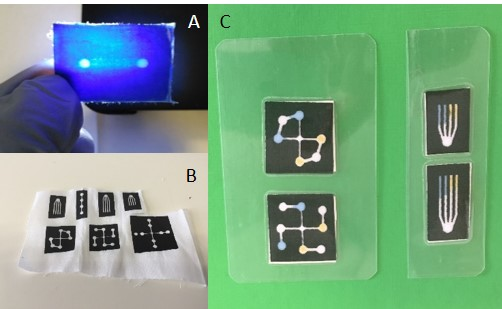
\includegraphics[width=\textwidth]{tela}
	\caption{ Prototipos de $\mu$CAD: A) serigrafía con cera; B) serigrafía con tintas vinílicas; C) laminado previo al uso.a}
	\label{fig:tela}
\end{figure}
Una reacción habitualmente utilizada para comprobar la validez de propuestas tanto de $\mu$PAD\cite{Ariza-Avidad2016} como de $\mu$TAD es la determinación enzimática de glucosa de tipo colorimétrico. Hemos estudiado algunas alternativas tanto para aumentar el tiempo de vida del dispositivo como para reducir su precio. Así la inclusión de glucosa oxidasa (GOx) y peroxidasa HRP en nanoflores de Cu$_{3}$(PO$_{4}$)$_{2}$ permite aumentar el tiempo de vida del dispositivo desde pocos días hasta 75 días. Las nanoflores bienzimáticas se sintetizan directamente sobre círculos de papel de 5 mm de diámetro que se utilizan como microrreactores en un diseño $\mu$PAD 3D (Figura \ref{fig:moneda}D)\cite{Ariza-Avidad2016}. La sustitución de un enzima por un mimético tipo nanozima permite eliminar componentes lábiles, en concreto la peroxidasa HRP y sustituirla por un MOF derivado de Fe$^{3+}$ y ácido tereftálico. El $\mu$PAD es de tipo monocanal (Figura \ref{fig:moneda}C), utiliza chitosan para inmovilizar los reactivos, situando GOx y el tampón en el canal de transporte y MOF y el cromógeno (TMB) en la zona de detección\cite{Ortiz-Gomez2018}.\\

Otra química utilizada se basa en compuestos luminiscentes, en concreto carbon dots (Cdots), cuya luminiscencia se mide como color (Figura \ref{fig:moneda}C). Estos nanomateriales son partículas cuasi esféricas de tamaño inferior a los 10 nm, muy solubles en agua, inertes y fácilmente modificables. Se han preparado por pirolisis a baja temperatura de ácido cítrico en presencia de polietilenimina para permitir la presencia de grupos carboxílico y amina en la superficie de las nanopartículas que permitan su funcionalización\cite{Pedro2014}.\\
 
El uso de Cdots en soporte papel presenta el inconveniente de que son arrastrados por la muestra originando una distribución irregular de la señal. El problema se resuelve mediante la unión covalente de los Cdots al papel a través de la química de vinilsulfonas, basada en una adición de Michael a grupos hidroxilo de la celulosa. El papel funcionalizado con Cdots se ha utilizado para la determinación de Cu$^{2+}$ fundada en la atenuación de luminiscencia que este origina. Una segunda estrategia se basa en la atenuación de la luminiscencia por efecto de átomo pesado, en concreto haciendo reaccionar el papel con Cdots inmovilizadas con ácido yodoacético, la cual se recupera por reacción con el analito glutatión.

%figura 5
\begin{figure}[h]
	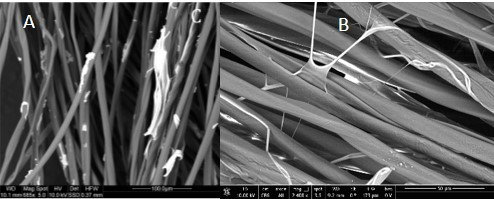
\includegraphics[width=\textwidth]{micro}
	\caption{Prototipos de $\mu$CAD: A) serigrafía con cera; B) serigrafía con tintas vinílicas; C) laminado previo al uso.}
	\label{fig:micro}
\end{figure}

En el caso de dispositivos$\mu$TAD, una de las químicas de reconocimiento utilizadas han sido las basadas en mecanismo ionóforo-cromoionóforo. Este mecanismo exige la inclusión de una membrana hidrófoba que imponga la condición de electroneutralidad requerida para que el reconocimiento de la especie buscada por el ionóforo (así éter dibenzo18-corona-6 para potasio\cite{Erenas2016} o calix[4]pirrol aril sustituido para creatinina) transcurra paralelo a la disociación del indicador de pH presente en la membrana. Para fabricar dicha membrana se añade sobre el hilo un volumen muy pequeño, del orden de 0,5 $\mu$L, de una disolución diluida conteniendo los reactivos necesarios que al evaporar el disolvente origina una fina red de filamentos (Figura \ref{fig:micro}).\\

La principal ventaja del uso de hilo de algodón como soporte para químicas ionóforo-cromoionóforo es que los tiempos de equilibrado, y por tanto de análisis, son sustancialmente menores que cuando se trabaja con la misma química en membrana, pasando de 3 minutos a 60 y 30 segundos, respectivamente, para potasio y creatinina, debido al aumento de superficie de la red de filamentos sensores en el hilo. Por otra parte, el volumen de muestra necesario es muy pequeño y, al incluir el tampón en el propio hilo, la muestra lo redisuelve y ajusta el pH. \\

El pequeño tiempo de reacción en hilo se ha observado en otras ocasiones como es el caso del dispositivo enzimático para la determinación de glucosa en sangre total una de cuyas principales novedades es el solo necesitar un minuto frente a los 10-15 minutos habituales de otros dispositivos colorimétricos, así como el permitir la separación del plasma de las partículas formes.\\

Una última estrategia en el uso de $\mu$TAD permite llevar a cabo la determinación electroquimioluminiscente de 2-dibutilaminoetanol. Para ello, se inmoviliza tris(2,2'-bipiridina) rutenio (III) en hilo de grosor dependiente de la cantidad necesaria para el análisis. Dicho hilo va laminado sobre la zona de trabajo de una celda electroquímica serigrafiada a la que se permite llegar la muestra mediante un hilo auxiliar (Figura \ref{fig:hilo}D).\\

\section{Análisis colorimétrico con smartphone}

Los dispositivos microfluídicos arriba descritos son de tipo óptico y, en concreto, colorimétricos. La señal obtenida será una variación del color o luminiscencia de la zona sensora o bien la aparición de color si no lo tenía inicialmente. Sin embargo, lo que se propone no es utilizar instrumentación convencional para medir una propiedad óptica o bien color, sino emplear dispositivos de electrónica de consumo que incluyan sensores de color como pueden ser escáneres, cámaras digitales, webcams o smartphones. La combinación de estos con los dispositivos microfluídicos capilares que responden a la muestra con color o cambio de color, da lugar a una imagen con información analítica latente que puede ser tratada fuera del laboratorio para atención domiciliaria, atención médica en áreas de bajos recursos o pruebas remotas en campo.\\

El uso de la electrónica de consumo que incluya sensores de color en Química Analítica es muy reciente. Prácticamente nació con el siglo XXI y su crecimiento es exponencial, siendo conocida como Química Analítica basada en visión artificial (Computer Vision-based Analytical Chemistry)\cite{Capitan-Vallvey2015}. Si consideramos los dispositivos usados en la bibliografía para adquirir la imagen, se observa un desplazamiento en el uso desde escáneres, webcams y cámaras digitales a smartphones. La razón es que los smartphones no solo permiten la adquisición de imágenes, sino su procesado para mejorar la imagen y calcular el ROI (Region Of Interest, zona de la imagen que contiene la información analítica), la obtención de las coordenadas cromáticas, el establecimiento del parámetro analítico, el cálculo de concentraciones, la transmisión de la información a una central remota donde pueda interpretarla y tomar decisiones un especialista y la geolocalización del punto de análisis, abriendo la puerta a minería de datos.\\

Por otra parte, los kits de herramientas de desarrollo de software que tienen los smartphones permiten la puesta a punto de aplicaciones específicas. Un ejemplo es el $\mu$PAD para la determinación de nitrito y pH antes citado\cite{Lopez-Ruiz2014} en el que tras reaccionar con la muestra de agua todo el tratamiento se hace con una aplicación desarrollada para Android  e instalada en el smartphone (Figura \ref{fig:app}A). La imagen se obtiene sujetando el móvil con la mano e iluminando el $\mu$PAD con el propio flash. Las marcas presentes en el dispositivo (triángulo y cuadrado) permiten que el software identifique la dirección y posición de las 7 zonas sensoras mas la zona de referencia, reduciendo la influencia de las variaciones iluminación, calculando los diferentes ROI, extrayendo las coordenadas cromáticas de cada analito (coordenada H del espacio de color HSV para pH y coordenada S para nitrito), y calculando las concentraciones respectivas a partir de las funciones de calibrado incluidas.\\

%figura 6

\begin{figure}[h]
	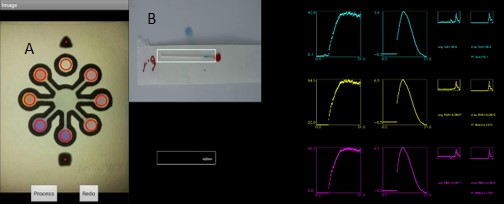
\includegraphics[width=\textwidth]{app}
	\caption{A) Captura de la aplicación para Android capaz de reconocer e identificar los ROI del sensor; B) imagen de la aplicación que analiza videos en tiempo real obteniendo el ROI y calculando sus coordenadas cromáticas.}
	\label{fig:app}
\end{figure}

En caso de no tener un ROI previamente definido o que se vaya a mantener fijo en una posición (Figura \ref{fig:app}B), se ha desarrollado una aplicación para Android que es capaz de detectarlo a medida que se vaya generando el color correspondiente a partir de un video. Se ha aplicado a la determinación de glucosa en sangre total antes comentada utilizando un $\mu$TAD que emplea muy bajos volúmenes de muestra, 3 $\mu$L, con un límite de detección de 28 mg/dL y una precisión del 10\%. En este caso, el análisis del ROI se hace al mismo tiempo que lo va detectando el smartphone trabajando en modo video, de manera que en el momento en que el parámetro analítico se hace constante, lo lleva a la función de calibrado para obtener la concentración de glucosa. De esta manera, el operador no necesita controlar el tiempo de medida ya que la aplicación toma el valor de señal de forma automática cuando esta se hace constante. Alternativamente, el software puede calcular la velocidad inicial de la reacción y utilizarla como parámetro analítico, haciendo posible la determinación cinética, de glucosa en este caso, en 10 segundos.






\bibliographystyle{unsrt}
\bibliography{Final}



	

\end{document}



